%=========================Preamble====================================%
\documentclass[12pt] {article}
\usepackage{times}
\usepackage[margin=1in,bottom=1in,top=0.6in]{geometry}

\usepackage{graphicx}
\usepackage{subfig}
\usepackage[usenames]{color}
\usepackage[]{todonotes}
\usepackage{blindtext}
\usepackage{listings}
\usepackage{hyperref}


%=========================Doc====================================%
\begin{document}
\title{Final Project - ECS 275\\
\vspace{2mm}
Accelerated Ray Tracing}

\author{Ahmed H. Mahmoud}
\date{June, 7th 2017} 
\maketitle

%=========================Intro====================================%
In this project we propose to accelerate ray tracing using two different method. In the first part we implemented efficient data structure in order to reduce the amount of computation needed to color a single pixel. In the second part we try to parallelize the computation using CUDA platform. Since the computation per pixel is independent from all other pixels, doing the computation in parallel sounds like an attractive option. We explore this idea and highlight the challenges on achieving speedup using CUDA.  

%=========================BVH====================================%
\section{Bounding Volume Hierarchy (BVH) Tree:}
We implemented the BVH tree on top of the base code used for the assignment one. We used the top-down construction style of the BVH tree. We start by assigning axis-aligned bounding volumes for the input object. Starting from the bounding volume that contains all objects, we split this box into two along one of the axes (we usually start by x-axis). The two resulting volumes are then split into two using different axes. We keep repeating this process until we reach volume that contain only less than two objects, thus binary tree. The traversal of the try is simple; starting with a ray coming out of a pixel, we go down the tree and intersect only the object(s) that intersect with the ray. 

\subsection{Experiments:}
We tested out implementation using the BVH on different models sets. We require from the user to input the objects that are supposed to be grouped in a single BVH tree. This requirement helps the computation in case of having one complex object of the same size of a simplified object (e.g., single sphere). Figure \ref{fig:bvh} show some examples of moderately complex scenes along with the timing with and without BVH tree. 

\begin{figure}[!tbh]
 \centering        
   \subfloat [1.32 sec - 43 sec]{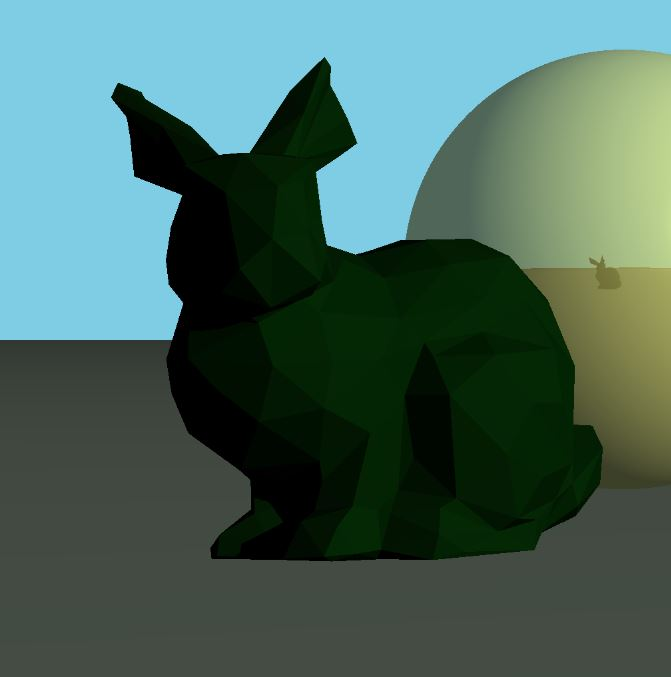
\includegraphics[width=0.33\textwidth]{bunny.JPG}}   
   \subfloat [1.71 sec - 34.7 sec]{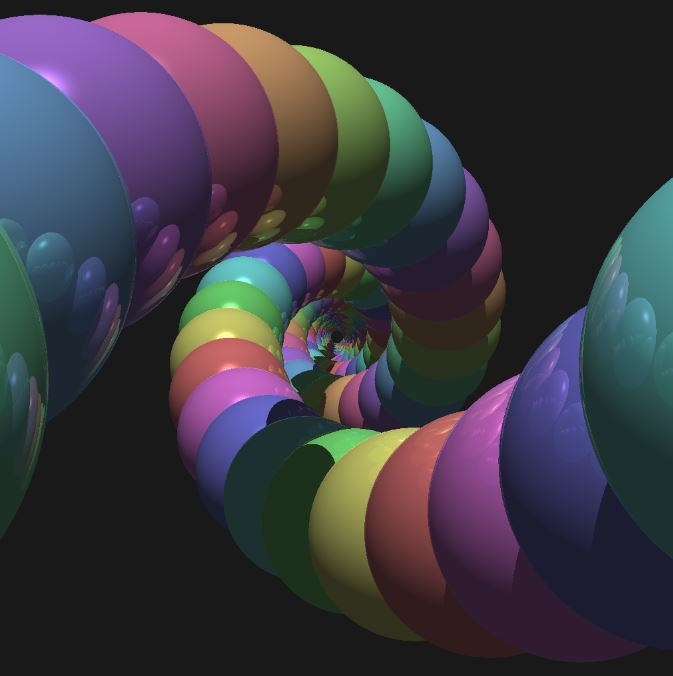
\includegraphics[width=0.33\textwidth]{spiral.JPG}}
   \subfloat [4.08 sec - 476 sec]{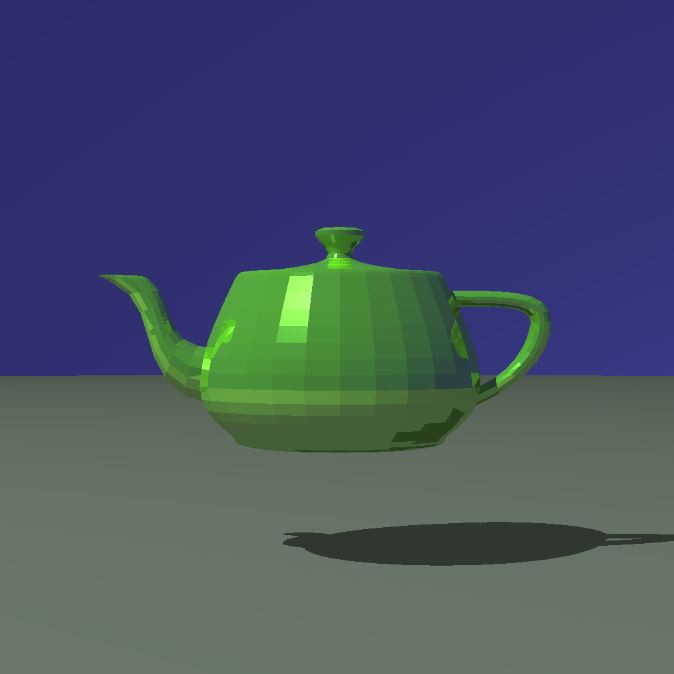
\includegraphics[width=0.33\textwidth]{teapot.JPG}}
   \caption{Example scenes along with the timing for rendering with (left) and without (right) BVH accelerated data structure.}
   \label{fig:bvh}
\end{figure} 

In order to assess the scaling of the speed up, we used the Bunny scene and isotropically subdivided each triangle into four. We did this four times to have four different resolution. We rendered each using accelerated BVH tree and plotted the timing in a graph as shown in Figure \ref{fig:study}. Even though both computation scale up linearly, but the gap between both implementation is huge. For example, the number of triangle in the final resolution is 47840 triangles which took the non-accelerated implementation about 55 minutes to render while it took BVH accelerated implementation 3.8 sec to render. 

\begin{figure}[!tbh]
 \centering        
   \subfloat {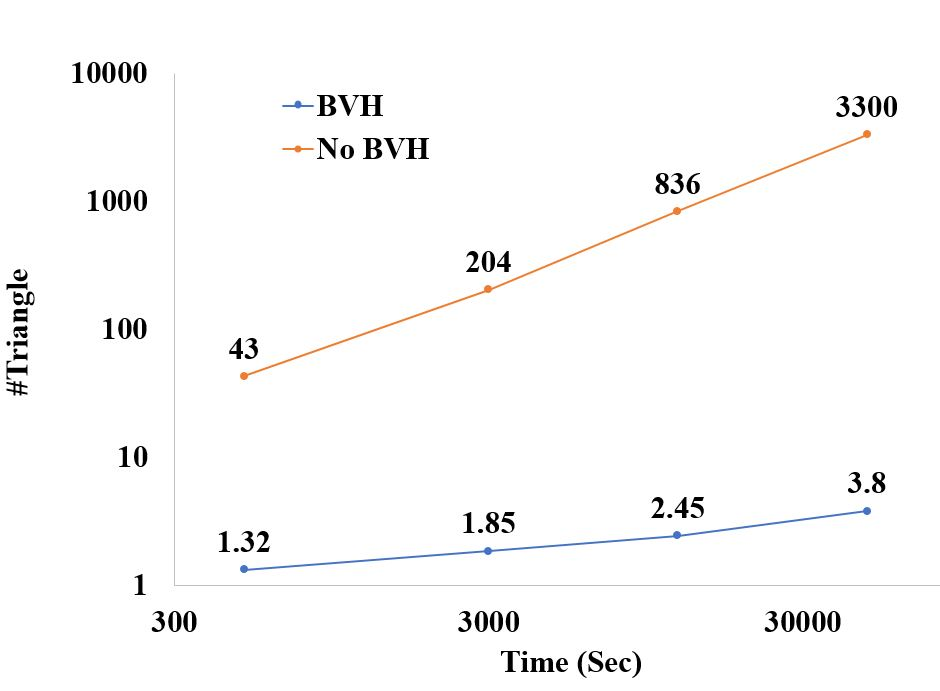
\includegraphics[width=0.6\textwidth]{bunny_study.JPG}}     
   \caption{Study of the scaling of the speedup on the Bunny scene using multiple resolution on a log-log scale.}
   \label{fig:study}
\end{figure}

%=========================CUDA====================================%
\section{CUDA Implementation:}

In this section, we turn into implementing the path tracing on CUDA. CUDA is a programming model that allows parallel execution through launching thousands of threads that can run in parallel. Using CUDA, we can write the same serial-like piece of code that will run on one thread. We then can launch as many threads as we would like. CUDA promises to schedule the threads across the compute resources as efficiently as possible. There are few precautions that must be taken into account that might slow down the computation. First, a thread should always seek to access contiguous chunks of memory. This is can be achieved by carefully lay out data in the memory. For path tracing, the data are the scene description. Thus, we can lay out all objects in the scene in \emph{struct} such that access a struct, we can get all information of the object (e.g., spatial position, material, color, speed, etc). Second, we should avoid thread divergence. Simply put, thread divergence is when two threads within one warp do different computations. A warp represents 32 threads. As long as threads within a warp do the same computation without branching, we can run them in parallel. Otherwise, their computation might be serialized leading to lower performance. 


CUDA style is attractive to do the path-tracing since the computation of one pixel is completely independent on other pixels. Figure \ref{fig:cuda} shows few examples of CUDA-implemented path-tracing. Unfortunately, the timing is not as promising as we hoped for. We assume that this is due to thread divergence since there is no guarantee that two threads within a warp will end up having the same number of bounces and hit the same object. 

\begin{figure}[!tbh]
 \centering        
   \subfloat [1.489 sec]{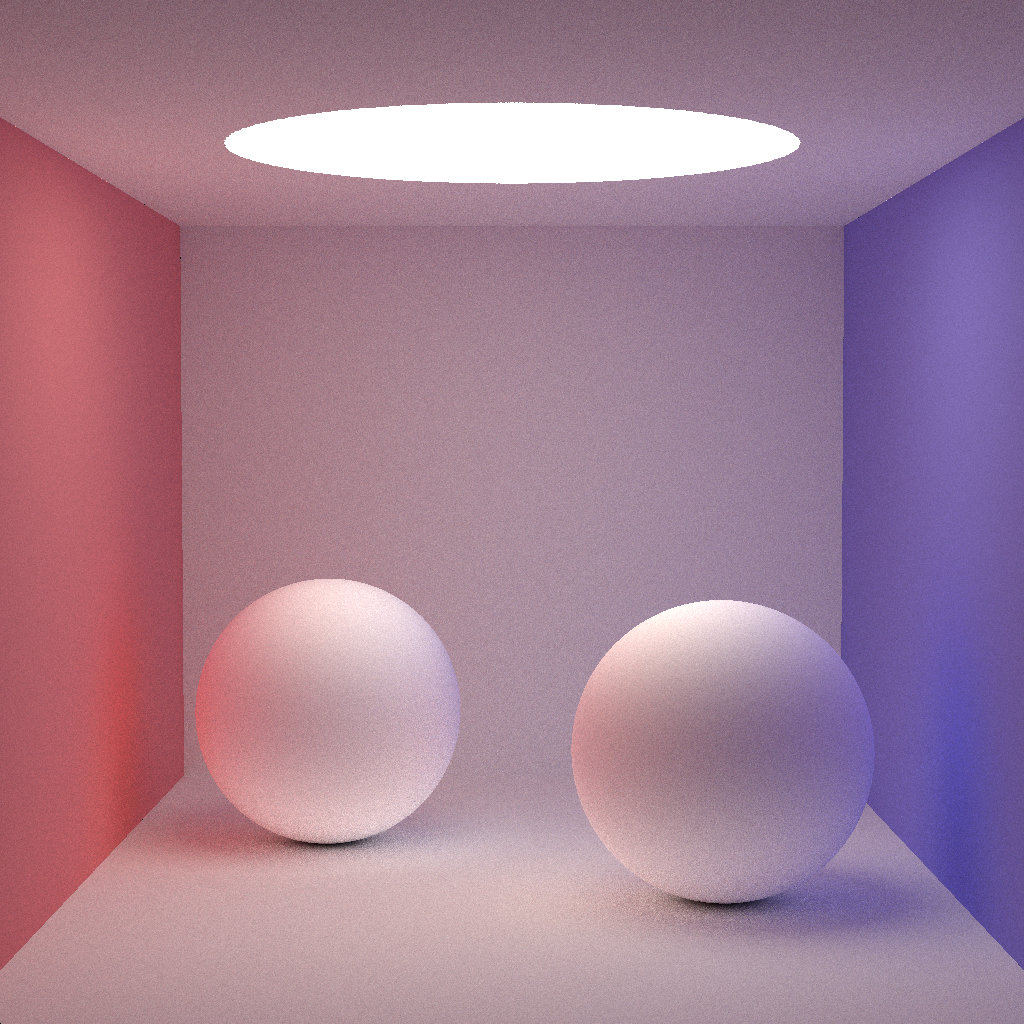
\includegraphics[width=0.24\textwidth]{cornell.png}}   
   \subfloat [1.4209 sec]{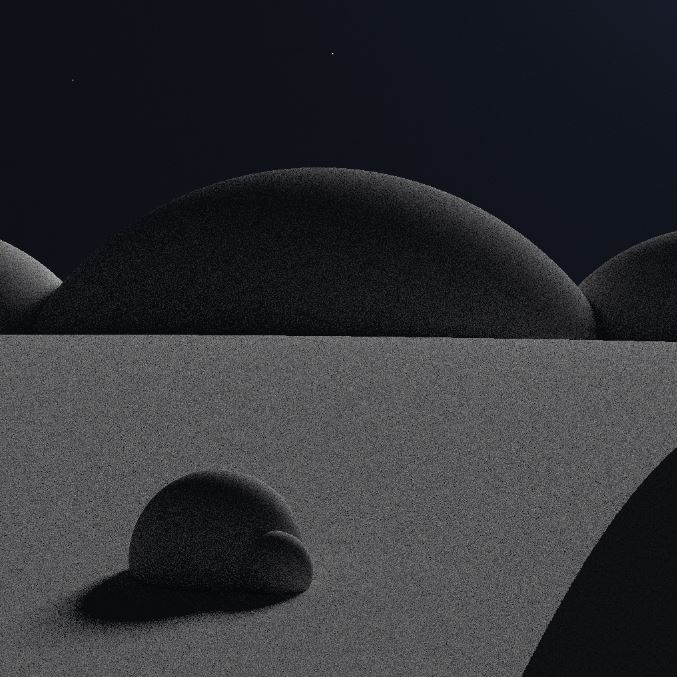
\includegraphics[width=0.24\textwidth]{nightsky.JPG}}
   \subfloat [2.283 sec]{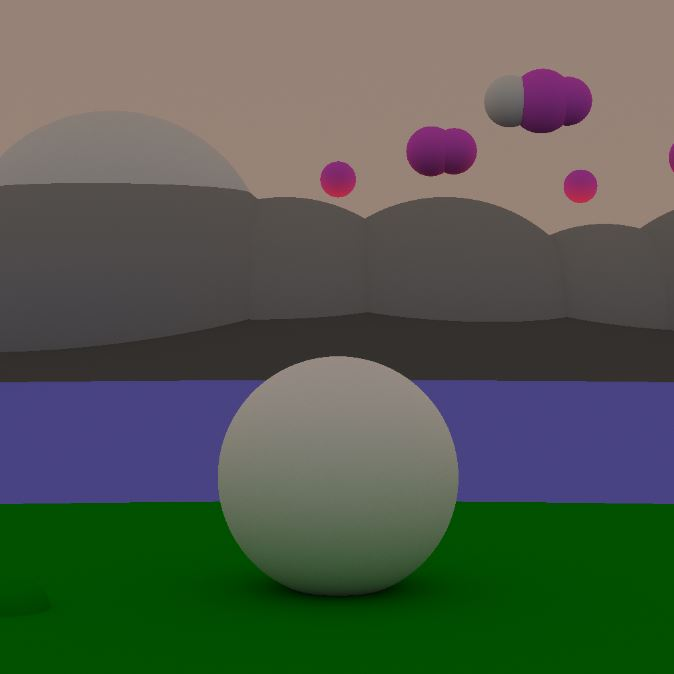
\includegraphics[width=0.24\textwidth]{vista.JPG}}
   \subfloat [1.686 sec]{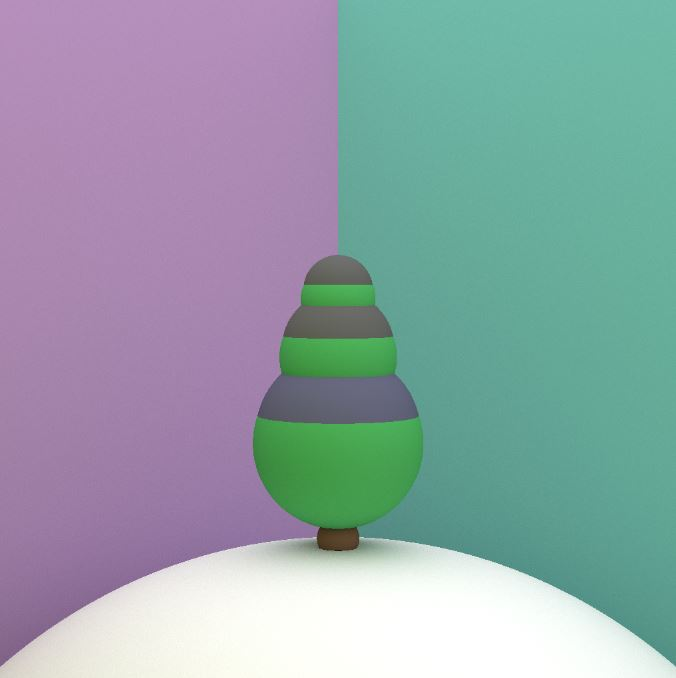
\includegraphics[width=0.24\textwidth]{tree.JPG}}
   \caption{Example scenes rendered using CUDA parallel implementation along with timing.}
   \label{fig:cuda}
\end{figure} 


%=========================Resoucres====================================%
The following is a list of website resources that were helpful in preparing this work:
\begin{enumerate}
\item \url{http://www.kevinbeason.com/smallpt/}
\item \url{http://raytracey.blogspot.com/}
\item \url{http://robbinmarcus.blogspot.nl/}
\item \url{http://www.cs.utah.edu/~acumming/cs6620/Computer_Graphics_II/Computer_Graphics_II_Spring_2009/Computer_Graphics_II_Spring_2009.html}
\end{enumerate}


\end{document}
